\chapter{Tecnologias}

\lipsum[1]

\section{Algor{\'i}tmo Gen{\'e}tico}

O processo evolutivo no campo da biologia é definido por
\citeonline{ridley2009evolucao} como uma mudança na forma e
nos comportamentos de uma determinada espécie ao longo das
gerações por um processo de seleção natural, “onde o indivíduo
mais bem adaptado sobrevive e deixa mais descendentes do que o
menos adaptado, o que conduz ao declínio de sua variedade ou
espécie, eventualmente conduzindo-a à extinção”
\cite{do2009alfred}.

A ideia de um AG é trazer todos esses conceitos embutidos na
biologia para modelos computacionais capazes de solucionar
problemas complexos de otimização por métodos
meta-heurísticos. Tais algoritmos não possuem um regra de
produção para seu desenvolvimento e implementação, sendo
apenas necessário abstrair a teoria biológica para o universo
da computação. Porém, de acordo com
\citeonline{mitchell1998introduction}, algumas
características, por convenção, sempre estão presentes, como,
por exemplo: populações de indivíduos, seleção dos mais aptos,
cálculo de função \textit{fitness}, crossovers para a reprodução e
mutações aleatórias.

\subsection{Indiv{\'i}duo e popula{\c c}{\~a}o}

Com base nas informações supracitadas é possível destrinchar
cada característica para melhor entendimento, iniciando pelo
elemento base do AG, o indivíduo.

Cada indivíduo de uma população é composto por uma sequência
de cromossomos. Cada cromossomo é composto por um conjunto de
valores binários. Cada valor binário desse conjunto é chamado
de gene. Então, com base nisso, é possível concluir que cada
indivíduo possui sua forma e comportamento ditados pelo seu
respectivo cromossomo e uma população é composta por um
conjunto de n diferentes cromossomos, como pode ser visto na
\autoref{fig_gene}.

\begin{figure}[htb]
        \centering
        \caption{\label{fig_gene}Gene, Cromossomo e População.}
        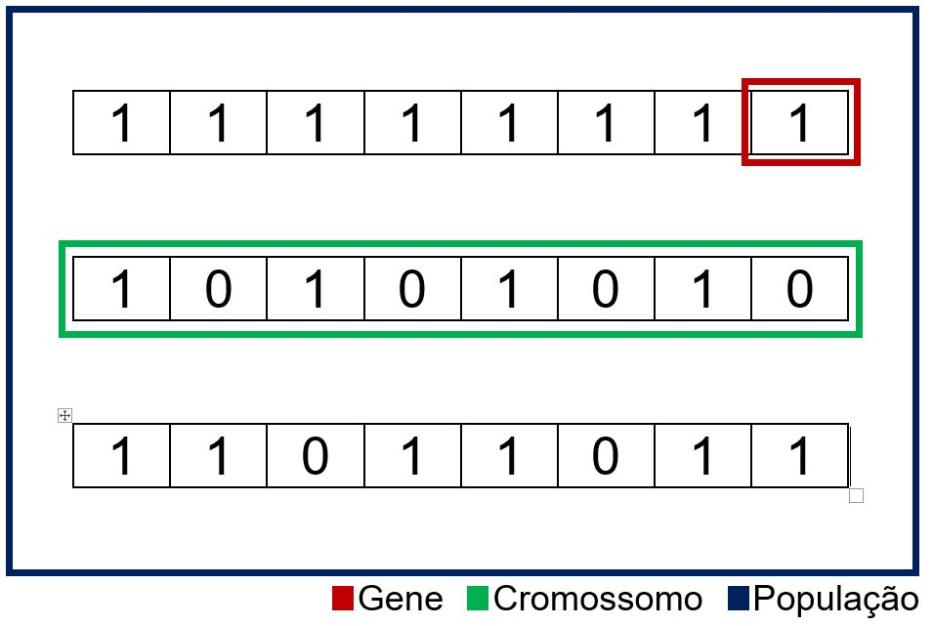
\includegraphics[width=0.7\textwidth]{images/gene.jpg}
        \legend{
                Fonte: Autoria Pr{\'o}pria.
        }
\end{figure}

\subsection{Reprodu{\c c}{\~a}o}

A reprodução é a parte considerada mais importante de um AG. É
nela que acontece a seleção e o cruzamento de cromossomos da
população com o intuito de gerar a evolução dos indivíduos e,
dessa forma, atingir o melhor resultado para a situação. 

Esse processo de reprodução é feito em etapas e ocorre sempre
que uma geração completa um ciclo de execução pré estabelecido
e há a necessidade de se criar uma nova geração. Esse processo
de reprodução somente chega ao fim quando o resultado gerado
pelo AG atinge o valor esperado, ou por uma condição de parada
definida anteriormente. 

Referente às etapas que constituem a reprodução, estão
inclusos os operadores de seleção, \textit{crossover} e
mutação.

\subsubsection{Sele{\c c}{\~a}o}

A etapa de seleção leva em consideração uma função chamada
\textit{fitness}, que é única para cada indivíduo de cada
geração após a execução de um ciclo. O cálculo desta função
varia e é definida de acordo com o problema que o AG está
inserido, utilizando dados essenciais para que seja possível
classificar que um cromossomo obteve um bom desempenho em uma
determinada situação. 

Com a \textit{fitness} de cada indivíduo calculado, “o
operador seleciona os cromossomos da população para a
reprodução, quanto maior o valor da função \textit{fitness}, maior a
chance desse mesmo cromossomo ser selecionado mais vezes para
reprodução” \cite{mitchell1998introduction}.  Além dos
indivíduos com melhor \textit{fitness}, são selecionados também, de
maneira aleatória, os demais cromossomos, para que a chance de
chegar em máximo local seja reduzida. A quantidade de
indivíduos selecionados, assim como a proporção de reprodução,
deve ser minimamente suficiente para que a geração seguinte
possua o mesmo tamanho da anterior.

\subsubsection{Crossover}

O \textit{crossover} é o responsável por gerar a evolução propriamente
dita. É durante essa etapa que os indivíduos recebem
características novas, porém, não necessariamente melhores.
Como dito anteriormente, o AG é um algoritmo meta-heurístico,
ou seja, busca otimizar problemas que não possuem
necessariamente apenas um resultado bom, mas sim diversos
resultados bons. Essa classificação se dá pelo “fato dos
cromossomos serem tratados apenas como sequências de bits sem
que sejam feitas inferências a respeito dos seus significados”
\cite{paulino2018}. Por isso, cromossomos anteriormente bons
podem perder suas qualidades e obterem resultados piores na
geração seguinte, porém, a vantagem é que o contrário também é
verdadeiro. Cromossomos ruins podem ganhar qualidades e
obterem resultados melhores.

Essas trocar de características e cruzamentos entre
cromossomos que é chamado de \textit{crossover}. A maneira com a qual o
\textit{crossover} é desenvolvido varia de acordo com a
situação em que o AG está inserido. Uma das maneiras mais
simples de realizar o \textit{crossover} é pegar dois cromossomos, ou
seja, duas cadeias binárias e realizar a inversão da primeira
metade do primeiro cromossomo com a segunda metade do segundo
cromossomo, como demonstrado na \autoref{fig_crossover} a
seguir.

\begin{figure}[htb]
        \centering
        \caption{\label{fig_crossover}Crossover entre dois cromossomos.}
        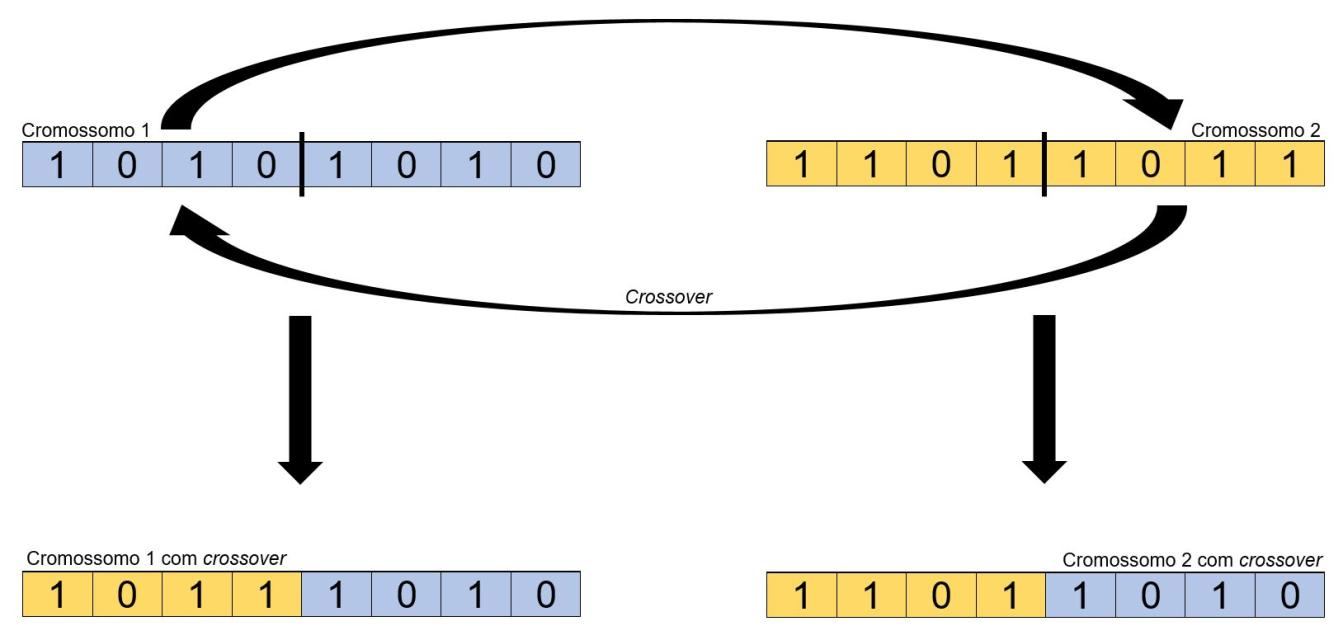
\includegraphics[width=0.7\textwidth]{images/crossover.jpg}
        \legend{
                Fonte: Autoria Pr{\'o}pria.
        }
\end{figure}

Dessa maneira ambos os cromossomos se beneficiam, ou não, das
características do outro sem perder todas as suas próprias
características. Esse processo cria uma nova população porém,
as características da geração anterior, por mais que
distribuídas entre os cromossomos, ainda estão presentes, só
organizadas de maneira diferente, não tendo uma evolução
propriamente dita, para isso que a próxima etapa, mutação, se
faz necessária.

\subsection{Muta{\c c}{\~a}o}

Após o \textit{crossover}, a nova população possui cromossomos
com genes organizados de maneira diferente. A mutação entra
para gerar uma alternância nos genes dos cromossomos
selecionados aleatoriamente com o intuito de gerar novas
características para a população. Porém, apesar de útil, a
mutação deve ser utilizada com cautela, tanto na questão de
cromossomos selecionados para mutação, quanto na quantidade de
genes selecionados por cromossomo, para que não haja
alterações descontroladas e nada produtivas para a resolução
do problema.

\section{Redes Neurais}

Uma Rede Neural é uma abstração computacional baseada no funcionamento do
sistema nervoso dos animais. Esse sistema é composto por diversos neurônios e
conexões entre esses mesmos neurônios para que sejam enviados sinais com
comandos para as demais células do organismo vivo. A capacidade de tomada de
decisão advém da organização dos neurônios e suas conexões formando uma grande
e complexa rede onde a menor unidade que pode ser encontrada é o neurônio
\cite{rojas2013neural}.

Um neurônio funciona recebendo informações fornecidas por demais neurônios,
gerando uma saída própria baseada nessas mesmas informações. No universo
computacional, o modelo com o objetivo de simular tais características de um
neurônio é chamado de \textit{perceptron}.

\lipsum[7]

\section{Neuroevolu{\c c}{\~a}o de Topologias Aumentantes}

\lipsum[2-6]
